\documentclass[]{article}

%packages
\usepackage{hyperref}
\usepackage{fancyhdr}
\usepackage{graphicx}
\usepackage{xcolor}
\usepackage{float}
\usepackage{booktabs}
\usepackage{subcaption}
\usepackage[format=plain, font=it]{caption}


\begin{document}

\begin{titlepage}

\newcommand{\HRule}{\rule{\linewidth}{0.5mm}} % Defines a new command for the horizontal lines, change thickness here

\center % Center everything on the page
 
%----------------------------------------------------------------------------------------
%	HEADING SECTIONS
%----------------------------------------------------------------------------------------

\textsc{\LARGE University of Twente}\\[1.5cm] % Name of your university/college
\textsc{\large Master Thesis}\\[0.5cm] % Minor heading such as course title

%----------------------------------------------------------------------------------------
%	TITLE SECTION
%----------------------------------------------------------------------------------------

\HRule \\[0.4cm]
\textsc{\Large Trust in automated decision making}\\[0.5cm] % Major heading such as course name
\textsc{\large How user's trust and perceived understanding is influenced by the quality of automatically generated explanations}\\[0.5cm] % Minor heading such as course title
\HRule \\[1.5cm]
 
%----------------------------------------------------------------------------------------
%	AUTHOR SECTION
%----------------------------------------------------------------------------------------


\begin{minipage}{0.4\textwidth}
\begin{flushleft} \large
\emph{Author:}\\
Andrea \textsc{Papenmeier} % Your name
\end{flushleft}
\end{minipage}
~
\begin{minipage}{0.4\textwidth}
\begin{flushright} \large
\emph{Supervisors:} \\
Dr. Christin \textsc{Seifert} \\% Supervisor's Name
Dr. Gwenn \textsc{Englebienne} % Supervisor's Name
\end{flushright}
\end{minipage}\\[2cm]


%----------------------------------------------------------------------------------------
%	DATE SECTION
%----------------------------------------------------------------------------------------

{\large \today}\\[2cm] % Date, change the \today to a set date if you want to be precise

%----------------------------------------------------------------------------------------
%	LOGO SECTION
%----------------------------------------------------------------------------------------


\includegraphics{img/UT_logo.png}\\ % Include a department/university logo - this will require the graphicx package
 
%----------------------------------------------------------------------------------------

\vfill % Fill the rest of the page with whitespace

\end{titlepage}

\begin{abstract}
	{\color{blue}Abstract and conclusion section will be written at the end.}
\end{abstract}

\newpage
\tableofcontents



\pagestyle{fancy}

\section*{Acknowledgements}
\section{Introduction}

State of the world \newline

machine learning employed for automatic decision-making

two good reasons to make those systems transparent:



The big BUT\newline
--- Xerox experiment [32] \newline
--> similar experiment but with automatic decision systems supporting a human (augmented intelligence)
                           
Research questions:\newline
\textbf{RQ 1:} What influence does the accuracy of an automatic decision system have on user's trust?\newline
\textbf{RQ 2:} To what extent is user's trust influenced by the truthfulness of automatically generated explanations?\newline
\textbf{RQ 3:} What role does the truthfulness of an explanation play for the user's perceived understanding?\newline

Therefore, we did\newline
The key findings are\newline
The contributions of this work are\newline
In HCI, the purpose of empirical contributions is to reveal formerly unknown insights about human behaviour in relation to information or technology.




\section{Background}

ML = ``representation + evaluation + optimization" [36] \newline
``The fundamental goal of machine learning is to generalize beyond the examples in the training set" [36] \newline


%------------------------------------------------------------------
\subsection{Transparency in AI}
``Machine learning is applied to the sorts of problems for which encoding an explicit logic of decision-making functions very poorly" [33] \newline
Opacity = intransparency: unclear ``how or why a particular classification has been arrived at from inputs" [33] \newline

Voluntary or involuntary intransparency due to [33]:
\begin{itemize}
	\item self-protection and censorship
	\item missing technical knowledge 
	\item curse of dimensionality vs. human cognitive abilities and intuition
\end{itemize}

Transparency via explainability [{\color{red}REF NEEDED}]

\paragraph{Definition Interpretability:}
\begin{itemize}
	\item Accurate proxy for model AND comprehensible for humans [3]
	\item Dimensions: scope (global vs local), time to understand (target user, use case), prior knowledge (user expertise), dimensionality, accuracy, fidelity (accuracy of explanation / accuracy of model), fairness, privacy, monotonicity, usability [3]
	\item operations can be understood by a human [10]
	\item descriptions understandable to humans [6]
	\item algorithm capability of producing patterns understandable to humans [16]
\end{itemize}
Interpretability vs. justification: Why it is a correct decision, not how it came along [10]\newline
Interpretability vs. explainability: Subgroup, showing reasons for behaviour [6] \newline 
interpretation = making inferences about underlying data [16] \newline
[31] argues that aiming for interpretability of algorithms suggests that there is an interpretability of human behaviour since humans can explain their actions and beliefs. Yet, the actual operations of the human brain remain opaque, which refutes interpretability [31]. \newline





%------------------------------------------------------------------
\subsection{Need for Explainability in AI}
``augmented intelligence" = machines supporting humans in cognitive tasks [16]\newline
xAI = communication with agents about their reasoning [12] \newline
xAI problems: reverse engineering (model, decision, visualisation/representation) and design of explanations [3] \newline
``Mixed initiative guidance" = human expert working alongside the ML system [4] \newline
xAI challenge: completeness and interpretability simultaneously (tradeoff), transparency vs. persuasiveness [6] \newline
xAI challenge: attention span of users \& perceived understanding rather than actual understanding [21] \newline
General trend: the higher the accuracy, the lower the explainability [15], or: complexity reduces interpretability [19] \newline
[29] user study shows that users do not necessarily perceive simpler systems as more understandably, presumably due to missing information\newline
Stakeholders: users and engineers, and at least one of those - explanations are user-dependent (not monolithic) [14] \newline
[17] found in a user study that users prefer more information and a higher information density (more soundness and completeness) as well as more general explanations rather than an explanation of each action. \newline
Including experts in the modelling and training process is not only a way to integrate expert knowledge that is otherwise difficult to model, but can also increase user trust [16]. \newline
Bad explanations ``provide an understanding that is at best incomplete and at worst false reassurance" [33] \newline

\paragraph{Goals of Explainability}
To achive transparency and accountability [14] \newline
Right for the right reasons: not enough to just be correct, the reasons need to be correct. Example of things going wrong without noticing: [56] \newline
for users: trust, for engineers: debugging and improving [14]\newline
trust when it comes to critical decisions (e.g. medical diagnosis) [29] \newline

user-related goals: \newline
Scrutability, trust, effectiveness, efficiency, satisfaction, persuasiveness [2] \newline
Explainability improves the user's confidence in the system, user's trust, user's judgement ability on prediction correctness, user satisfaction, user acceptance [10] \newline
acceptance, trust, perceived competence [59] \newline
acceptance, appropriate trust [38] \newline

\paragraph{Issues with Opacity}
\begin{itemize}
	\item high cost of errors in high-risk domains [2] [8] [17]
	\item human safety in safety-critical tasks [6] [15]
	\item automated discrimination [2], biased training data [6] [15] [24]
	\item censorship [2]
	\item development: fine-tuning parameters with trial-and-error [4]
	\item imperceptibly altered input data or altered model: criminals / hackers [6]
	\item unintuitive systematic errors [6] [56] [24]
	\item regulations: right to explanation [1] [6] [8]
	\item source of knowledge that should be accessible if needed [8] [15]
	\item (inappropriate) trust into the system (either too much or too little) [15] [14] [17] [24]
	\item implementation involves a lot of human work [33]
\end{itemize}
need dependent on consequences of classification results [15]:
\begin{itemize}
	\item \textbf{no need} for interpretability if no consequences arise from faulty decisions
	\item interpretability is \textbf{beneficial} if consequences for individuals arise from faulty decisions
	\item interpretability is \textbf{critical} if serious consequences arise from faulty decisions
\end{itemize}
need also dependent on user role [38] \newline

\paragraph{Barriers to Interpretability}
intentional concealment, lack of technical expertise, computational complexity vs. human-scale reasoning abilities [1] \newline
minimum explainability: how features (values) relate to predictions [1] \newline

\paragraph{Regulations}
General Data Prodection Regulation (GDPR): law about processing of personal (related to identifiable person) data, no matter if manually or automatically processed [1] \newline
Sensitive data / protected traits: race, ethnicity, religion, nationality, gender, sexuality, disability, marital status, age [2] \newline
Real-life data contains society's structures and biases, and as classification means separation into groups based on that data, biases are taken into the model [1] \newline
\begin{itemize}
	\item minimal interpretation: delete sensitive data from dataset
	\item maximum interpretation: delete sensitive data and correlated variables from dataset
\end{itemize}
``right to explanation" [1], argument against such interpretation [58] and positive interpretation [37]. Key issue: ``data subjects receive meaningful, but properly limited, information" [58] is ambiguous, plus no clear definition of explanation, meaningful, and information. Summary: Precedents are needed to clarify the boundaries.\newline
Problem with explanations: ML algorithms show statistical correlation, not causality [1]\newline


\paragraph{Accountability}
information worth disclosing for more accountability [2]:
\begin{itemize}
	\item human involvement: who controls the algorithm, who designed it etc., leading to control through social pressure
	\item data statistics (accuracy, completeness, uncertainty, representativeness), labelling \& collection process, preprocessing of data
	\item model: input, weights, parameters, hidden information
	\item inferencing: covariance matrix to estimate risk, prevention measures for known errors, confidence score 
	\item algorithmic presence: visibility, filtering, reach of algorithm
\end{itemize}

\paragraph{Persuasiveness}
persuasiveness of explanation != actual explanation [10]\newline
``High-fidelity explanations, also referred to as faithful, have a strong correspondence between the explanation model and the underlying machine learning model" [51]\newline
``[Persuasive explanations] are less faithful to the underlying model than descriptive explanations in a tradeoff for more freedom on the explanation complexity, structure, and parameters. This freedom permits explanations better tailored to human cognitive function, making them more functionally interpretable." [51]\newline
``Descriptive explanations best satisfy the ethical goal of transparency" [51]\newline






%------------------------------------------------------------------
\subsection{Application Areas}

\subsubsection{Application Areas}
decisions that affect people’s lives in critical domains like criminal
justice, fair lending, and medicine. [52]\newline
safety-critical industries (self-driving cars, robotic assistants, personalised medicine) [3]\newline

sensitive data processed by algorithms (banks, insurances, health data) [3]\newline

scientific research (making discoveries by understanding data) [3]\newline

individual performance monitoring, health care, economic situation analysis, personal preferences \& interests, location \& movement [1]\newline

replacing human decision making in advertising, recommendations, finances (loans) [6] \newline

health care, recommender systems, planning, HRI [15]\newline

medicine, finances, criminal justice [19] \newline

education, health care, manufacturing, retail, when machine learning based support systems are used [16] \newline

high-risk domains: medical diagnosis, terrorism detection [24] \newline

``socially consequential mechanisms of classification and ranking" [33] \newline

spam detection, finances (fraud detection, loan), search engines, news trends, marketing, insurance [33] [36] \newline

\subsubsection{Exemplary Failures}
examples of failures due to missing explanation:
[3]:
\begin{itemize}
	\item St Georges hospital - racist application procedure 
	\item COMPASS crime prediction - racist against blacks (counterargument made in [55]: ``group differences in scores may reflect true differences in recidivism risk")
	\item Amazon prime district selection - defavorising neighborhoods with ethnic minorities
	\item Automated target identification - decision driven by weather condition
	\item Animal race 
	\item Mortgage rates of major US banks rate very differently - sign for bad algorithms?
\end{itemize}
``Discrimination, is at some level, inherent to profiling: the point of profiling is to treat some people differently" [57]:
\begin{itemize}
	\item Discrimination of women: ads of higher-paid jobs more often shown to men than to women (but no reason given, may be intentional)
\end{itemize}
[54]
\begin{itemize}
	\item researcher group is the main reason for variance, not classifier etc., hence human bias in ML
\end{itemize}
[14]
\begin{itemize}
	\item Google Flue Trends: systematic modelling error 
\end{itemize}







%------------------------------------------------------------------
\subsection{Explanations}
Explanation = reasons or justification for an action or belief [14]\newline

Function of explanations:\newline
\begin{itemize}
	\item prediction of consequences of (similar) events in the future [11] [5]
	\item control of events  [5]
	\item building and refining inner knowledge model [5]
	\item restauration / prevention of states or events [11]
	\item comparison of methods [11]
	\item reproduction of states or events [11]
	\item assigning guilt [11] [5]
	\item justification [11] [5]
	\item persuasion [5]
	\item pleasure / appreciation [11]
\end{itemize}

\subsubsection{Human-Human Explanations}
explanations are not mental model but rather the interpretation of relations [11]\newline
explanations are less general than theories and are application-focussed [11] \newline
explanations are a cognitive and social process: The challenge of explaining includes finding a complete but compressed explanation, and transferring the explanation from the explainer to the explainee [5].\newline
Complete explanation == all relevant causes explained [5] \newline

Explanation aspects [11]:
\begin{itemize}
	\item causal pattern content: common-cause, common-effect, linear chain, homeostatics
	\item explanatory stance types: mechanical, design, intention stance [5]. Atypical stances can lead to distorted understanding.
	\item explanatory domain: different fields have different preferences of explanation types
	\item social-emotional content: can alter acceptance threshold and influence recipient's perception of explained event 
\end{itemize}
What constitutes a \textbf{good explanation}? [11] describes good explanations as being non-circular, showing coherence, and having a high relevance for the recipient. Circularity are causal chains where an effect is given as cause to itself (with zero or more causal steps in between). Explanations can, but do not have to, explain causal relations [11]. Especially in the case of machine learning algorithms, the learned model shows correlation, not causation. Explanations for statistical models therefore cannot draw on typical causal explanations as found in human-human communication {\color{red}[REF NEEDED]}. The probabilistic interpretation of causality comes closest to the patterns learned in statistical models: If an even $A$ caused an event $B$, then the occurrence of $A$ increases the probability of $B$ occurring. Statistical facts are not satisfactory elements of an explanation, unless explaining the event of observing a fact [5]. Arguably, this holds true for statistical learning. Coherence refers to the systemacity of explanation elements: good explanations do not hold contradicting elements, but elements that influence each other [11]. Finally, relevance is driven by the level of detail given in the explanation. The sender has to adapt the explanation to the recipient's prior knowledge level and cognitive ability to understand the explanation [5], which can mean to generalise and to omit information - [11] calls this adaptation process the ``common informational grounding". The act of explaining also includes a broader grounding of shared beliefs and meanings of events and the world [5]. The ``compression problem" poses a major challenge in constructing explanations for humans. Humans tend to not comprise all possible causes and aspects of the high-dimensional real world in an explanation, suggesting that there are compression strategies (on the sender's side) and coping strategies (on the recipient's side) in place [11]. \newline
[5] notes that besides presenting likely causes, and coherence, a good explanation is simple and general. The latter two characteristics refer to the agreement widely accepted in science that a simple theory (or, in this case, an explanation) is favoured over a more complicated theory if both explain an equal set of events or states.\newline
[21] defines a good explanation as sound, complete, but nor overwhelming. While soundness refers to the level of truthfulness, completeness describes the level of disclosure [21]. In order to avoid overwhelming the explainee, the informational grounding process takes place, i.e. a common understanding of related elements and an adaptation of the explanation's detailedness to the explainee's knowledge level.\newline

Generally, the more diverse the given evidence, the higher the recipient's \textbf{acceptance} of the explanation [11].\newline

Cultural differences exist for the preference of an explanation type, although all explanation types can be understood [11].\newline

Humans build \textbf{mental models} of the world, a mental representation of events or elements. Mental models are needed to explain and predict. We do not need to have complete, holistic mental models in order to use an artifact, but a ``functional" model is needed to tell us how to use and make use of it, while a ``structural" model stores information about the composition and how it is built [21]. \newline

mindlessness and explanations [32]\newline

\paragraph{Explanation Types}
associations between antecedent and consequent, contrast and differences, causal mechanisms [10] \newline
material cause, formal / categorical cause, efficient cause, final cause [5] \newline


\subsubsection{AI-Human Explanations}
Focus:\newline
[10]:
\begin{itemize}
	\item feature-level: feature influence, intersection of actual \& expected contribution per feature
	\item sample-level: explanation vector, linguistic explanation for textual data using BOW, subtext as justification for class (trained independently), caption generation 
	\item model-level: rule extraction, prototypes \& criticism samples representing model, proxy model (inherently interpretable) with comparable accuracy (NOTE: supposedly meant decision generation, not simple accuracy)
\end{itemize}
single focus: feature-based explanation best for recommender systems (as compared to similar previous decisions and similar neighbor decisions) [10] \newline
[4]:
\begin{itemize}
	\item understanding and reassurance (right for the right reasons)
	\item diagnosis (of errors, inacceptable performance or behaviour)
	\item refinement (improving robustness and performance)
\end{itemize}
[6]:
\begin{itemize}
	\item representation of data \& features
	\item processing of data (operations)
	\item explanation generation (within model)
\end{itemize}
[5]:
\begin{itemize}
	\item computational / operations level
	\item representational level
	\item hardware level
\end{itemize}
[8]:
\begin{itemize}
	\item learning algorithm behaviour
	\item model parameters
	\item model itself
	\item representation
\end{itemize}
[15]:
\begin{itemize}
	\item within algorithm, directly based on model
	\item feature-based
	\item secondary, add-on explanation system separate from learning algorithm
	\item representation
\end{itemize}
[14]:
\begin{itemize}
	\item inner workings for transparency
	\item post-hoc prediction visualisation, e.g. heat maps
\end{itemize}
[16]:
\begin{itemize}
	\item dataset / features
	\item optimizer / learning algorithm
	\item model 
	\item prediction / result
	\item evaluator
\end{itemize}

\textbf{Explanation selection}: it is not possible to show every case, parameter, feature importance to the user, therefore a selection of exemplary cases needs to be made [24]. Global explanation can originate from a set of representative cases [24].



\subsubsection{When to explain?}
[15] stresses that different explainability needs call for different timings of the explanation. Showing the explanation \textbf{before} a classification or generation task is useful for justifying the next step or explaining the plan. {\color{green}\textbf{During} a task, information about the operations and features can help identifying errors for correction and foster trust.} Explaining the results of a task \textbf{after} the process is useful for reporting and knowledge discovery.



\subsubsection{Explanation Systems}
For models that are not inherently interpretable, the explanation can only be an approximation and cannot be complete (definition of non interpretable) [5]. There can be approximations for the computation / operations detecting properties and categorisations, and approximations of the decision behaviour [5].\newline

counterfactual explanation [12] with fact \& foil \newline
[4] for overview over solutions for understanding, diagnosis, refinement \newline
[6] for overview of solutions for explaining features, operations, generative explanations \newline
[16] for solutions for dataset, optimizer, model, predictor and evaluator \newline
[14] for set of programs (MYCIN, NEOMYCIN, CENTAUR, EES) that try to model explanations alongside with system \newline
[19] presenting the L2X system\newline
[24] Explanation software: LIME, ELUCIDEBUG

For feature-based models, [19] suggests salience map masks on input features, comparable cases (input and output) as reference (or very dissimilar cases as counterfactuals), and mutual information analysis per feature. For the latter, they use the Kullback-Leibler divergence to calculate the mutual information of two vectors: Learning to explain (L2X).\newline

Inherently interpretable / transparent models:
\begin{itemize}
	\item decision trees (graphical representation), rules (textual representation), linear models (feature magnitude and sign) [3]
	\item shallow rule-based models, decision lists, decision trees, feature selection, compositional generative models [10]
	\item 
\end{itemize}

[{\color{red}REF NEEDED}] add-on and post-hoc systems might be good as explaining, but this fact in itself does not guarantee a sound, i.e. truthful, explanation, ``however plausible they appear" [31]. \newline

[15] suggests to develop a new class of learning algorithms that have an inherent ``explainability hyperparameter" to achieve high accuracy AND high explainability.\newline

[36] argues that most high-dimensional real-world application data is ``concentrated on or near a lower-dimensional manifold" [36], dimension reduction techniques like PCA or other feature selection algorithms can therefore be used to overcome the curse of dimensionality. \newline

\textbf{explanations for texts}:
[7] solution to recent development in text mining, where texts are represented in a high-dimensional vector space (e.g. fasttext, word2vec) and classified with neural nets. Compared to BOW/SVM, the W2V/CCN they used yields equally good results, because the CNN is better at identifying characteristic words.\newline
[19] designed a system that uses deep neural networks for classification and mutual information for getting the input feature importance (in their case, single words). \newline

\textbf{Relevant words}: A word is relevant to the text if removing it from the texts and classifying again results in a decrease of the classification score across all texts







%------------------------------------------------------------------
\subsection{Explanation Evaluation}
[6]:
\begin{itemize}
	\item application grounded: true context, true task, users
	\item human-grounded: usability tests, human performance tests
	\item functionally grounded: no users, proxy
\end{itemize}
[8] evaluation of model interpretability:
\begin{itemize}
	\item heuristics: number of rules, number of nodes, minimum description length (model parameters)
	\item generics: ability to select features, ability to produce class-typical data points, ability to provide information about decision boundaries
	\item specifics: user testing / perception (BUT: evaluation of visuals and perceived model rather than actual model), e.g. by measuring accuracy of prediction, answer time, answer confidence, understanding of model
\end{itemize}
[15] rather combination than only a single one:
\begin{itemize}
	\item algorithm performance score
	\item user performance score
	\item user satisfaction score 
\end{itemize}







%------------------------------------------------------------------
\subsection{Trust in AI}
[25] notes that there exists no precise definition of trust in the field of computer science\newline

[TRUST 02] examined the concept of trust in close relationships and define it as the willingness to put oneself at a risk and believing that the other will be benevolent. They grouped aspects of interpersonal trust into a model with three components: faith, dependability, predictability [TRUST 02]. \newline
Placed in agent, not a characteristic inherent to an agent [TRUST 02]\newline
Trust is a subjective experience rather than objectively measurable [TRUST 05] [23]. \newline
dynamic: evolves as relationship matures [TRUST 02]\newline
attribution of characteristics, e.g. dependability (repeated confirmation in risky situations), reliability (consistency or recurrent behaviour) [TRUST 02]\newline
inappropriate trust can be harmful [17]\newline
Trust as experience, trustworthiness is the characteristic and in case of computer programs consists of factors such as security, privacy, dependability, usability, correctness [TRUST 05] [TRUST 06]. Trust relates to the assurance that a system performs as expected [TRUST 05]. \newline
Trust in a system can be misused: e-crime with negative side effects, e.g. data misuse [TRUST 05]. \newline 

\subsubsection{Gaining User Trust}
Trust factors: appeal, competence (privacy, security, functionality), transparency, duration (relationship, affiliation), reputation [23] \newline
Concerning algorithms, users can put global trust into the system, which means trusting the model itself. Trust can also be assigned locally, into an individual decision. [24] \newline
Trust dimensions of web systems: target (the entity being evaluated), representation (encoding of trust via social warranty, certificates, etc.), method (security), management (the entity putting trust into the system), computation (evaluation metric), purpose [25] \newline
For classification: expectation mismatch leads to direct decrease in trust [30], strength of decrease depends on the type of mismatch. Data-related mismatch weights less strongly than logic-driven mismatch. [30] \newline 
[31] argues that trust in machine learning algorithms also depends on the characteristics of misclassified cases. He points out that an automatic system can be considered trustworthy if it behaves exactly like humans, i.e. it misclassifies the same data points as a human and is correct on those cases that a human would also correctly classify [31].

\subsubsection{Trust Evaluation}
[23]: using experts to assign a weighted label to each element on a website or GUI and calculating a score
\begin{itemize}
	\item [-1] irritant
	\item [1] chaotic
	\item [2] assuring
	\item [3] motivating
	\item [0] not present
\end{itemize}
But user study showed that experts find it problematic to assign discrete trust values. The advantage of this approach, however, is that it is possible to compare multiple websites [23]. \newline
user study with closed and open questions [24]:
\begin{itemize}
	\item Do you trust this algorithm to work well in the real world?
	\item Why do you trust this algorithm to work well in the real world?
	\item How do you think the algorithm distinguished between the two classes?
	\item How certain are you of the correctness of your explanation? 
\end{itemize}
[TRUST 02] develops a trust scale with 26 items, each belonging to one of the three trust factors (faith, dependability, predictability). \newline
[TRUST 01] describes online trust (websites) as developing from external factors (website's reputation, navigational architecture, user's prior experience) as well as perceived factors (credibility, ease of use, risk) \newline
{\color{green}``willingness to accept a computer-generated recommendation is considered a proxy measure of trust" [38] }

\subsubsection{Perceived Understanding}
Perceived understanding important for trust (rather than actual understanding):\newline
``Findings show that the transparent version was perceived as more understandable and perceived understanding correlated with perceived competence, trust and acceptance of the system. Future research is necessary to evaluate the effects of transparency on trust in and acceptance of user-adaptive systems" [59] \newline
Most questionnaires use factual statements to investigate perceived understanding. Participants rate the statements according to their confidence of understanding [UND 03] [UND 07] or directly their subjective understanding [UND 01] [UND 02] [UND 04] [UND 05]



%------------------------------------------------------------------
\subsection{Use Case Scenario}
definition of offensive language [34] \newline








%------------------------------------------------------------------
\subsection{Summary}
Summary\newline
\begin{itemize}
	\item summary scenario
	\item systems
	\item evaluation of explanations and of trust
\end{itemize}
Hypotheses














\section{Method}
Intro

Similar to the copy machine experiment. Comparison can be drawn because willingness to follow a recommendation is presumably somewhat similar to willingness to comply with a request 

explanation: minimum explanation setup suggested by \cite{goodman16eu} explaining how input features relate to the prediction.

\subsection{Use Case Scenario}
definition of offensive language [34] \newline
hate speech detection systems \newline

\subsection{Evaluation setup}

Two evaluations: 
\begin{itemize}
	\item explanation evaluation (generics, ability to select truthfully important words from texts) to asses whether the explanations are ``good" in terms of truthful
	\item user evaluation to assess trust and perceived understanding
\end{itemize}








\section{Materials}
\addtocontents{toc}{\protect\setcounter{tocdepth}{2}}

{\color{blue}This section is still in bullet-points state and formulations/wording is not final!}\medskip \newline
Intro: this section is for the technical documentation of the data preprocessing, classifier implementation, explanation generation and validation. 


\subsection{Dataset}

\subsubsection{Dataset Construction}
The original dataset was collected by Davidson et al. \cite{davidson2017automated} for their research on defining and differentiating hate speech from offensive language. They constructed a dataset with offensive Tweets and hate speech by conducting a keyword search on Twitter, using keywords registered in the hatebase dictionary\footnote{https://www.hatebase.org}. The timelines of Twitter users identified with the keyword search were scraped, resulting in a dataset of over 8 million Tweets. They selected 25 000 Tweets at random and had at least 3 annotators from Figure Eight\footnote{https://www.figure-eight.com} (formerly Crowd Flower) who labelled each Tweet as containing hate speech, offensive language, or neither. They reached an inter-annotator agreement of 0.92 \cite{davidson2017automated}. The dataset is publicly available on GitHub\footnote{https://github.com/t-davidson/hate-speech-and-offensive-language}.\newline
The biggest class in the dataset are the offensive language Tweets (77\%), while non-offensive Tweets represent 17\%, and hate speech 6\% of the dataset. \newline
For our research, we are only interested in offensive and not offensive Tweets. We therefore excluded Tweets labelled as hate speech for the further construction of our dataset. We produced a balanced dataset by selecting only Tweets with the maximum inter-annotator agreement from each of the two remaining classes, and randomly drew Tweets from the bigger class (offensive Tweets) until the size of the subset was equal to the size of the smaller class (non-offensive Tweets). Table \ref{tab:StatsDataset} presents statistical information about the resulting dataset.
%-------------------------------------------------------
\begin{table}[!ht]
	\centering
	\begin{tabular}{lll}
		\hline
		\textbf{} & \textbf{Not Offensive Class} & \textbf{Offensive Class} \\ \hline
		Size (absolute) & 4,162 & 4,162 \\
		Size (relative) & 50.00\% & 50.00\% \\
		Total words & 58,288 & 61,504 \\
		Unique words & 6,437 & 9,855 \\
		\begin{tabular}[c]{@{}l@{}}Average words\\per Tweet\end{tabular} & 14.00 & 14.78 \\ \hline         
	\end{tabular}
	\caption{Statistical characteristics of the constructed dataset}
	\label{tab:StatsDataset}
\end{table}
%-------------------------------------------------------




\subsubsection{Dataset Preprocessing}
To prepare the data to be used in a machine learning application, we adopt the following preprocessing steps (see section \ref{subsubsec:tweet_cleaning}) in chronological order:
\begin{enumerate}
	\item Conversion of all texts to lower cases
	\item Replacement of URLs by a dummy URL (``URL")
	\item Replacement of referenced user names and handles by a dummy handle (``USERNAME")
	\item This dataset encodes emojis in unicode decimal codes, e.g. ``\&\#128512;" for a grinning face. In order to keep the information contained in emojis, each emoji is replaced by its textual description (upper cased and without whitespaces to ensure unity for tokenizing)\footnote{https://www.quackit.com/character\_sets/emoji/}.
	\item Resolving contractions such as ``we're" or ``don't" by replacing contractions with their long version\footnote{https://en.wikipedia.org/wiki/Wikipedia:List\_of\_English\_contractions}.
	\item This dataset uses a few signifiers such as ``english translation" to mark a Tweet that has been translated to English, or ``rt" to mark a Retweet (i.e. a response to a previous Tweet). Since those information have been added retrospectively, we discard them here and delete the signifiers from the texts.
	\item Replacement of all characters that are non-alphabetic and not a hashtag by a whitespace
	\item Replacement of more than one subsequent whitespace by a single whitespace
	\item Tokenization on whitespaces
\end{enumerate}
After training the classifiers, the URL and username tokens are replaced by a more readable version (``http://website.com/website" and ``@username", respectively) to make it easier for participants of the user study to envision themselves in the scenario of a social media administrator reading real-world Tweets. Replacing the tokens by their original URLs and usernames would give the participants more information than the classifiers had; we therefore chose to use a dummy URL and username.\medskip\newline

Following the preprocessing steps, the following Tweet is processed from its original form:
\medskip \hrule \medskip
\begin{verbatim}
	"@WBUR: A smuggler explains how he helped fighters along the \end{verbatim}\begin{verbatim}"Jihadi Highway": http://t.co/UX4anxeAwd"
\end{verbatim}
\medskip \hrule \medskip
into a cleaned version:
\medskip \hrule \medskip
\begin{verbatim}
@username a smuggler explains how he helped fighters along the \end{verbatim}\begin{verbatim}jihadi highway http://website.com/website
\end{verbatim}
\medskip \hrule \medskip





\subsection{Classifier}
Intro

\paragraph{Good System}
L2X 

\paragraph{Medium System}
Logistic Regression with binary (1 / -1) coefficients to bring down accuracy towards the needed 0.7. In a way, \cite{klenner2018offensive} does the same, but identify the ``sign" (offensiveness) of words not by using a logistic regression classifier. In the end, it leads to the same result: with binary coefficients, the label corresponds to the class that has the most words in the sentence.

\paragraph{Bad System}
Inverse L2X



\subsection{Explanations}
reference to section \ref{subsubsec:explanation_systems}: explanations for text via highlighting of important features (here: words). 

\paragraph{Good System}
L2X mutual information

\paragraph{Medium System}
randomly choosing k words from the words with positive (offensive) or negative (not offensive) class. With logreg, a sentence of n words, all n could have the same sign (i.e. adding towards the same class). But since we use the binarised version of the coefficients (to bring down accuracy), we are confronted with n selected words. We need to choose k words to be consistent with the explanations of the L2X classifier. We therefore randomly draw k words from the set of words with the same sign.

\paragraph{Bad System}
Inverse good system



\subsection{Graphical User Interface}
\begin{itemize}
	\item the ``environment": administration tool
	\item visualisation of the decisions
	\item visualisation of the explanations (why changing text colour, why those two colours, why not gradient)
\end{itemize}

\begin{figure} [H]
	\centering
	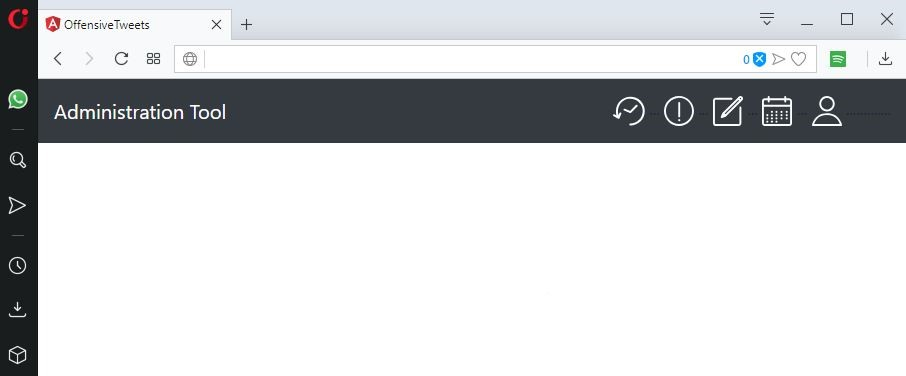
\includegraphics[width=0.8\textwidth]{img/administrationTool.JPG}\\
	\caption{Screenshot of the ``Administration Tool" to support the scenario of a social media administrator}
	\label{fig:admin_tool}
\end{figure}
\begin{figure} [H]
	\centering
	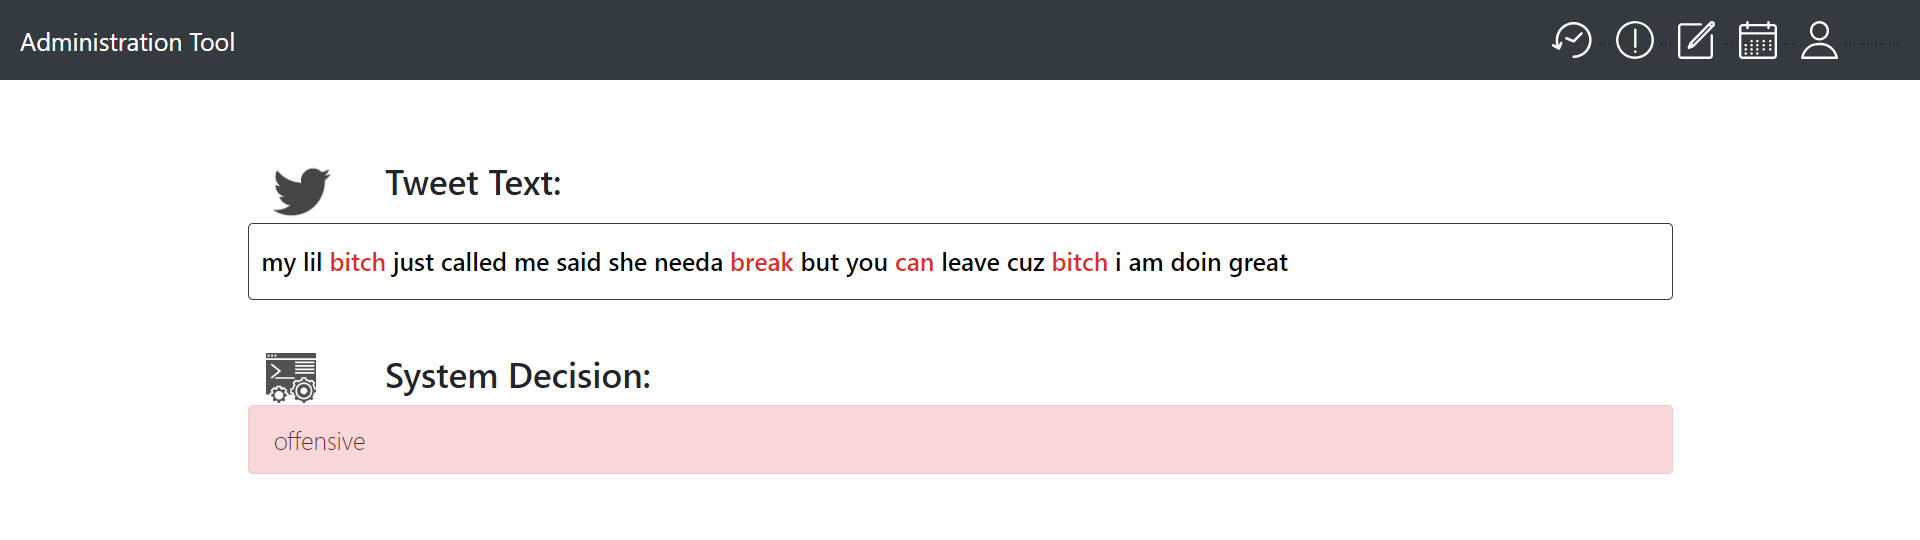
\includegraphics[width=0.8\textwidth]{img/pg_2_12.PNG}\\
	\caption{Screenshot of the ``Administration Tool" showing an offensive Tweet with explanation for its decision}
	\label{fig:admin_tool_offensive}
\end{figure}
\begin{figure} [H]
	\centering
	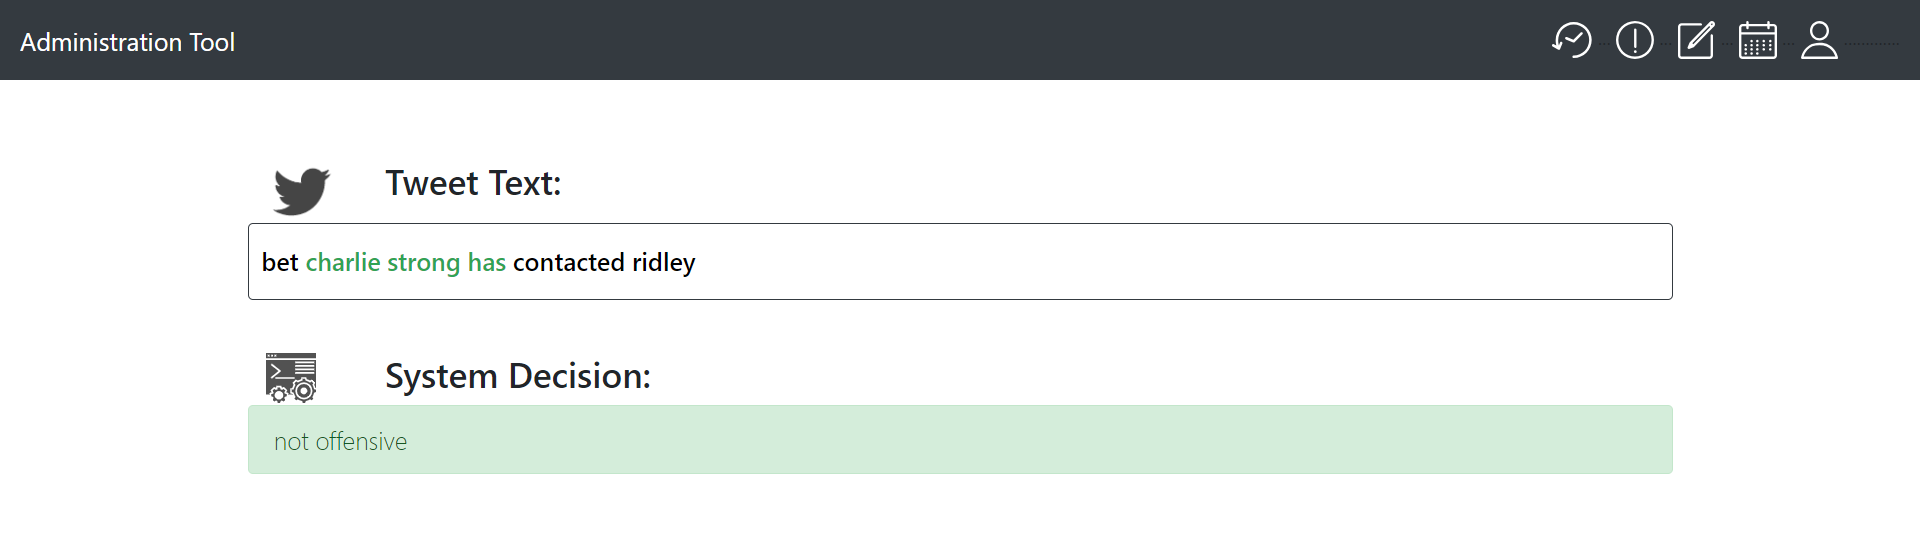
\includegraphics[width=0.8\textwidth]{img/pg_2_0.PNG}\\
	\caption{Screenshot of the ``Administration Tool" showing a non-offensive Tweet with explanation for its decision}
	\label{fig:admin_tool_not_offensive}
\end{figure}



\subsection{Subset Sampling}
For evaluating the different system-explanation conditions, users have to experience the system. However, it is not feasible to present them with the complete testeset, since it has a size of 1665 Tweets. Consequently, a subset of Tweets needs to be drawn from the testset, with a size that a human observer can understand and process within the time frame of a user study.\newline
We furthermore aim to find 10 suitable subsets and assign participants randomly to one of the subsets, in order to reduce possible side effects from biases specific to single Tweets.\newline
There are several requirements for the subsamples, originating from the conflict of reducing the sample for a human observer, yet still yielding a good representation of the testset and classifier:\newline
\begin{itemize}
	\item A class balance of the true labels similar to the testset, 
	\item a balance of correctly to incorrectly classified data points similar to the classifier's performance on the complete testset, 
	\item no overlap of Tweets within the set of 10 subsets,
	\item a feature distribution as close to the feature distribution in the complete testset.
\end{itemize}
We set the subsample size to 15 Tweets, which is enough to show accuracies to the first decimal place, yet assumably not too much to process for an observer in a user study.\newline
To create a subset, 15 data points are randomly drawn from the testset. \newline
First, the class balance of the subset is calculated. The difference to the class balance of the whole testset needs to be smaller than 0.1.\newline
Additionally, for each classifier in the user study, the prediction accuracy on the subset is compared to the prediction accuracy on the complete testset. If, for all classifiers, the difference is smaller than 0.1, the next check is performed.\newline
To ensure the uniqueness of the subsets, the randomly drawn Tweets are compared with the content of previously found subsets. The subset is only accepted if none of the contained Tweets appear in any previously found subset.\newline
In the last step, the feature distribution of the subset is tested against the features of the complete testset using the \textit{Kullback-Leibler Divergence} (KLD) metric. As the focus is directed towards the explanations (i.e. the highlighted words within a Tweet), only the explanations are used to examine the feature distribution. First, the feature distribution of the complete testset is calculated by constructing a word vector with tuples of words and their respective word counts. The word counts are divided by the total amount of words in the set, such that the sum of regularised counts equals 1. Next, a copy of the word vector is used to count and regularise the word frequencies in the subset. The result are two comparable vectors, yet the vector of the subset is very likely to contain zero counts for words that appear in the complete set but were never selected as explanation in the subset. Since the KLD uses the logarithm, it is undefined for zero counts. We use Laplace smoothing with k=1 to handle zero counts. For each classifier, the KLD is calculated and summed to a total divergence score for the subset.\newline
We generate a quantity of 100 such subsets and order them by their KLD sum. The 10 subsets with the smallest score are chosen as the final set of subsets.\newline




\subsection{Explanation Evaluation}
\label{subsec:expleval}
experiments to validate whether the explanations we generate are actually ``good" explanations and those generated with the random method are actually ``bad" explanations.


\subsubsection{Evaluation 1: Accuracy on Reduced Texts}
For each system, take generated explanations of Tweets in the test set, reduce the text to the selected words, and feed the ``reduced Tweets" into the system. Hypothesis: If the words are very informative for the classifier, the accuracy would not change. The new accuracy should then be close to the old accuracy.\newline
\begin{figure}[H]
	\centering
	\begin{subfigure}[b]{0.4\textwidth}
		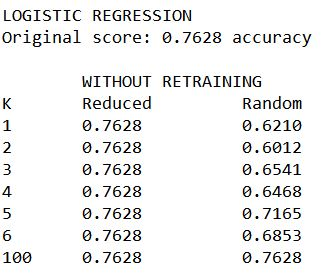
\includegraphics[width=\textwidth]{img/expleval1_logreg.JPG}
	\end{subfigure}
	\begin{subfigure}[b]{0.4\textwidth}
		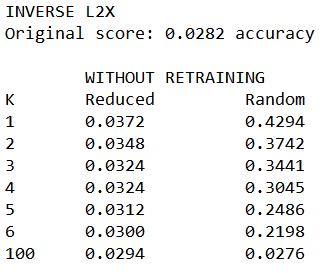
\includegraphics[width=\textwidth]{img/expleval1_invL2X.JPG}
	\end{subfigure}
	\caption{Results for evaluation of explanation experiment 1}
	\label{fig:results_expleval1}
\end{figure}
Problem: Tweets are very short, which is why the information density is high. Even when using only a single word randomly drawn from the text, the accuracy is 0.64, which is close to the medium classifier. It is therefore difficult to interpret the results for the medium classifier (0.76). Furthermore, we do not know if the Tweets have classified the same, or if only the accuracy is the same, but the mistakes were made on different Tweets. We therefore need to evaluate the ability to reproduce the very same classifications (evaluation 2).


\subsubsection{Evaluation 2: Ability to Reproduce Classifications}
For each system, divide the dataset in 5 chunks. Use each chunk once as testset and the remaining chunks as training set. This way, we get predictions and generated explanations for each data point in the dataset. Use the reduced version of the dataset with the predictions as truths to repeat the procedure of evaluation 1. Hypothesis: If the selected words are very informative for the classifier's prediction, the very same predictions can be reproduced with the reduced dataset. Since we take the predictions of the classifier on the non-reduced dataset as ``truth", the accuracy should be close to 1.0 .
\begin{figure}[H]
	\centering
	\begin{subfigure}[b]{0.4\textwidth}
		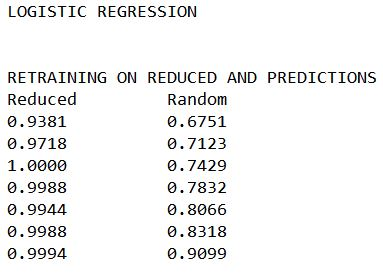
\includegraphics[width=\textwidth]{img/expleval2_logreg.JPG}
	\end{subfigure}
	\begin{subfigure}[b]{0.4\textwidth}
		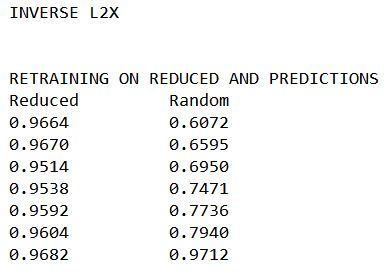
\includegraphics[width=\textwidth]{img/expleval2_invL2X.JPG}
	\end{subfigure}
	\caption{Results for evaluation of explanation experiment 2}
	\label{fig:results_expleval2}
\end{figure}



\subsection{Subset Evaluation}
same as previous section, but with the filtered subsets, basically. And on ``perfect" classifier. For k=4, because we use k=4 for final explanation generation.



\addtocontents{toc}{\protect\setcounter{tocdepth}{3}}
\section{Results}
The following section presents the results of the user study. We examined perceived understanding, self-reported trust and an implicit trust measure via the willingness to follow a classifier's recommendation. For each topic, we give the mean score, standard deviation, as well as a comparison of all conditions in a 9x9 matrix.\newline
The matrices show each condition checked for significant difference with every other condition. The colour scale is a visualisation of the differences in means ($\bar{x}_{row} - \bar{x}_{column}$ ), with negative differences coloured in red and positive differences in green. Per cell, the net difference values are displayed as well. The significance test results are added with asterisks, where one asterisk means significant at $\alpha=0.05$ significance level, while two asterisks denote significance at $\alpha=0.01$ significance level.\newline 

\paragraph{Demographics}
In total, 327 participants took part in the main user study with an average age of 29.4 years (SD = 8.8), a gender balance of 56\% (females) to 43\% (males) and two participants reporting the third gender. 87\% of the participants were recruited via ``Prolific", while 36 participants enlisted on ``SurveyCircle". 57\% self-assessed their level of English to be equivalent to a native speaker, 23\% as advanced (C1), 14\% as upper-intermediate (B2), and 5\% as lower than that. All participants claimed to be ``fluent" in English. The exclusion criteria (passed attention check and completion of whole questionnaire) invalidated 41 data points, resulting in 286 valid cases. More detailed statistics about the participants' backgrounds are given in appendix B.\newline

\paragraph{Perceived Understanding}
As figure \ref{fig:results_matrix_understanding} shows, users of the system with a very good classifier and no explanation report the highest perceived understanding. For the very good and the medium classifier, giving no explanations for the decisions leads to a higher perceived understanding than delivering placebic, i.e. random, explanations. In general, users have more confidence in their understanding of the system for the very good and medium classifiers as compared to the bad classifier. One condition, however, does not lead to significantly higher scores than the bad classifier: for the medium classifier with random explanations, users reported the same understanding as for the bad classifier with no explanations. Concerning the bad classifier, giving a truthful explanation for the decision leads to the lowest perceived understanding.

\begin{table}[h]
	\makebox[\textwidth][c]{
	\begin{tabular}{lrr|lrr|lrr}
		\textbf{Condition} & \textbf{Mean} & \textbf{SD} & \textbf{Condition} & \textbf{Mean} & \textbf{SD} & \textbf{Condition} & \textbf{Mean} & \textbf{SD} \\ \midrule
		super-good & 3.944 & 0.915 & super-rand & 3.729 & 0.860 & super-no & 4.147 & 0.701 \\
		medium-good & 3.818 & 0.825 & medium-rand & 2.944 & 0.963 & medium-no & 3.700 & 0.690 \\
		bad-good & 2.465 & 1.201 & bad-rand & 2.500 & 1.138 & bad-no & 2.944 & 1.152 \\ \bottomrule
	\end{tabular}}
	\caption{Mean scores for perceived understanding measure}
	\label{fig:results_table_understanding}
\end{table}

\begin{figure}[H]
	\makebox[\textwidth][c]{
		\begin{minipage}[t]{0.65\textwidth}
			\centering
			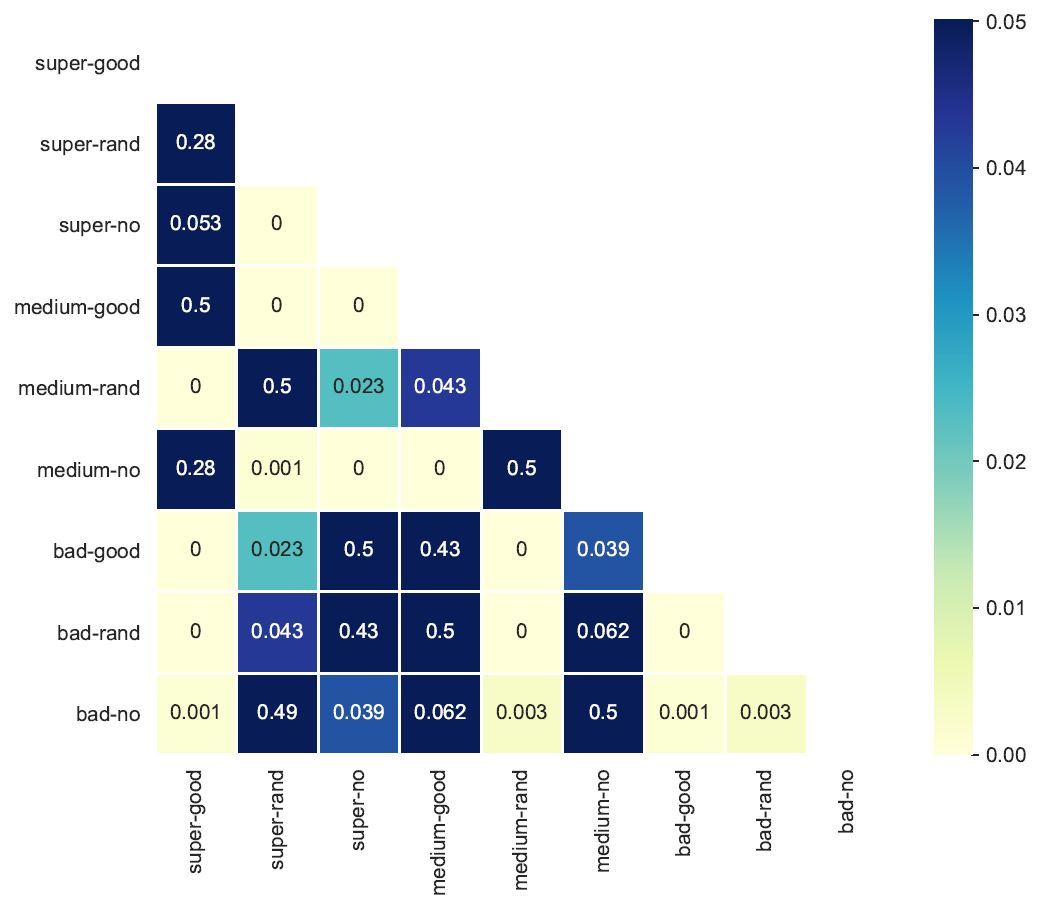
\includegraphics[width=\textwidth]{img/results_matrix_understanding.JPG}
			\caption{Comparison of perceived understanding scores ordered by classifier, value reporting difference of means ($\bar{x}_{row} - \bar{x}_{column}$ ), asterisk reporting significance (* significant at $\alpha=0.05$, ** significant at $\alpha=0.01$)}
			\label{fig:results_matrix_understanding}
		\end{minipage}%
		\hspace{5mm}
		\begin{minipage}[t]{0.65\textwidth}
			\centering
			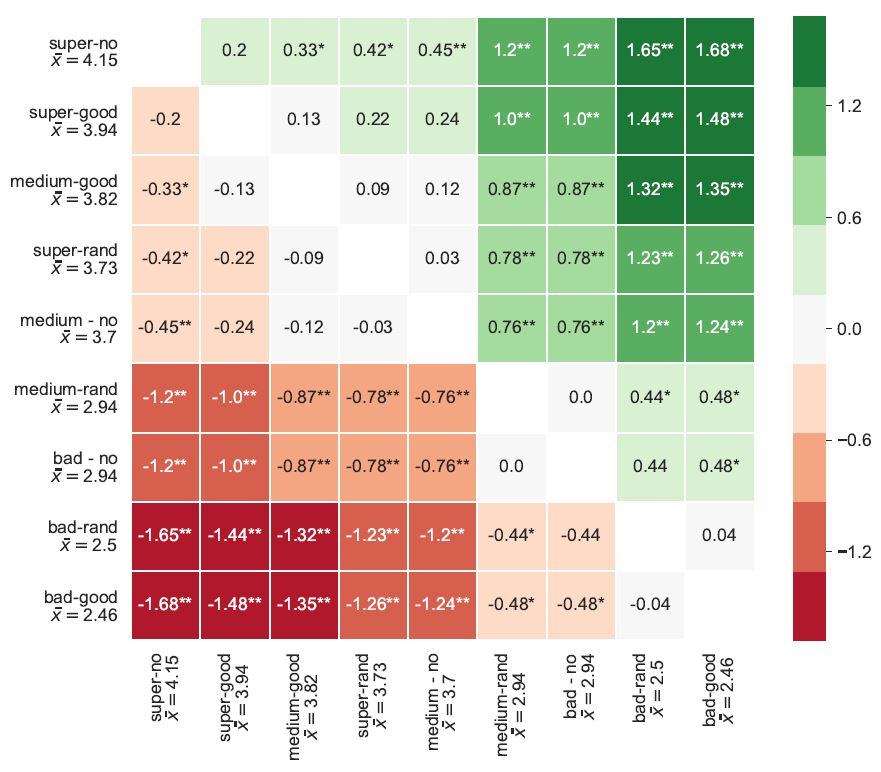
\includegraphics[width=\textwidth]{img/results_matrix_understanding_reordered.JPG}
			\caption{Comparison of perceived understanding scores ordered by explanation type, value reporting difference of means ($\bar{x}_{row} - \bar{x}_{column}$ ), asterisk reporting significance (* significant at $\alpha=0.05$, ** significant at $\alpha=0.01$)}
			\label{fig:results_matrix_understanding_reordered}
		\end{minipage}}
\end{figure}


\paragraph{Trust Questionnaire}
The self-reported trust scores show similar results as the perceived understanding: Besides the medium classifier with random explanations, all systems lead to significantly more trust than the systems employing the bad classifier. The explanations do not play a role regarding user's trust when the bad classifier is used. Looking at the medium classifier, the random explanation leads to a lower trust score than no explanation and a good explanation, with no difference between the latter two. The most trust is evoked by the very good classifier without explanations, significantly more than for any other condition. There is no significant difference between the very good classifier with explanations and the medium classifier with meaningful explanation. For both the bad classifier and the very good classifier, the condition without any explanation again led to the highest scores within the same classifiers. The detailed results are presented in figure \ref{fig:results_matrix_trust}.

\begin{table}[h]
	\makebox[\textwidth][c]{
		\begin{tabular}{lrr|lrr|lrr}
			\textbf{Condition} & \textbf{Mean} & \textbf{SD} & \textbf{Condition} & \textbf{Mean} & \textbf{SD} & \textbf{Condition} & \textbf{Mean} & \textbf{SD} \\ \midrule
			super-good & 2.682 & 0.400 & super-rand & 2.679 & 0.482 & super-no & 2.995 & 0.512 \\
			medium-good & 2.633 & 0.482 & medium-rand & 2.211 & 0.509 & medium-no & 2.630 & 0.459 \\
			bad-good & 1.917 & 0.428 & bad-rand & 1.951 & 0.403 & bad-no & 2.018 & 0.546 \\ \bottomrule
	\end{tabular}}
	\caption{Mean scores for self-reported trust measure}
	\label{fig:results_table_trust}
\end{table}

\begin{figure}[H]
	\makebox[\textwidth][c]{
		\begin{minipage}[t]{0.65\textwidth}
			\centering
			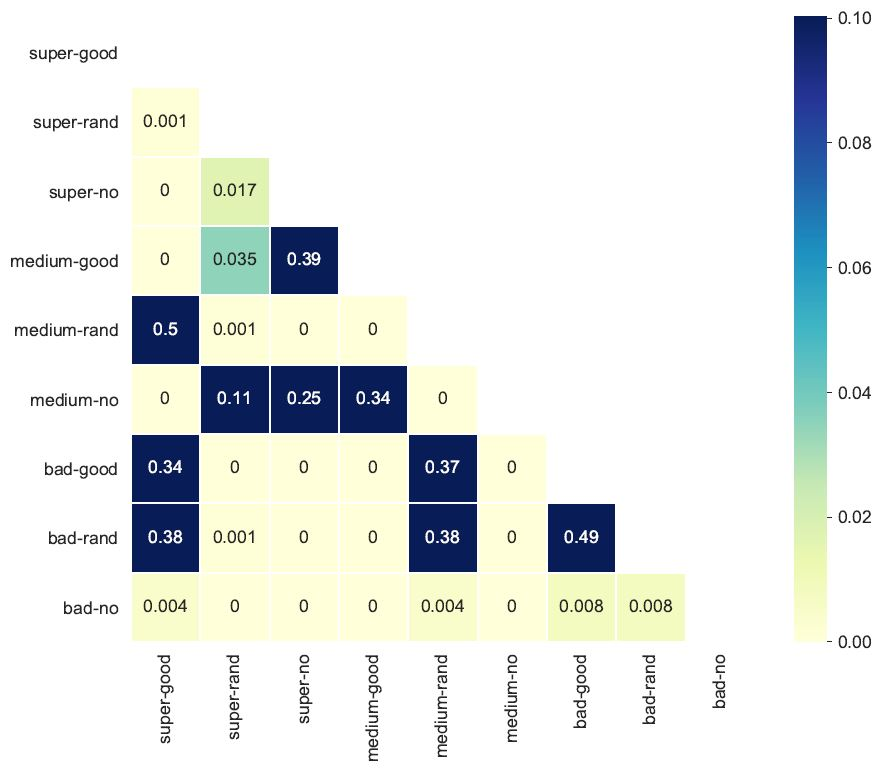
\includegraphics[width=\textwidth]{img/results_matrix_trust.JPG}
			\caption{Comparison of trust scores ordered by classifier, value reporting difference of means ($\bar{x}_{row} - \bar{x}_{column}$ ), asterisk reporting significance (* significant at $\alpha=0.05$, ** significant at $\alpha=0.01$)}
			\label{fig:results_matrix_trust}
		\end{minipage}%
		\hspace{5mm}
		\begin{minipage}[t]{0.65\textwidth}
			\centering
			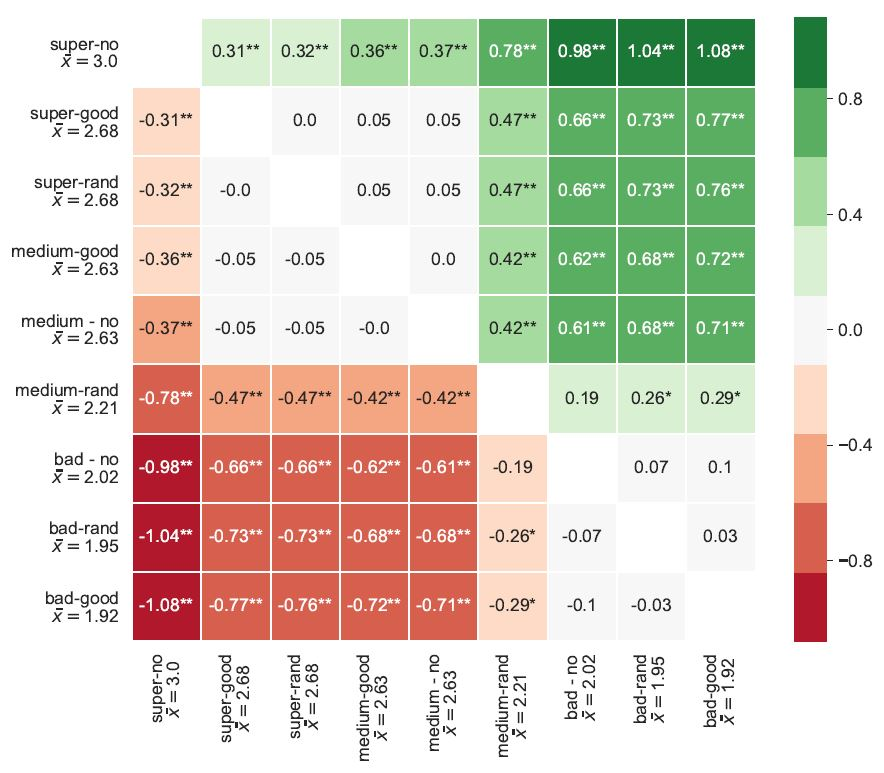
\includegraphics[width=\textwidth]{img/results_matrix_trust_reordered.JPG}
			\caption{Comparison of trust scores ordered by explanation type, value reporting difference of means ($\bar{x}_{row} - \bar{x}_{column}$ ), asterisk reporting significance (* significant at $\alpha=0.05$, ** significant at $\alpha=0.01$)}
			\label{fig:results_matrix_trust_reordered}
	\end{minipage}}
\end{figure}


\paragraph{Observed Trust via Proxy}
The second trust measure uses a proxy to determine the trust a user puts into a system: the willingness to follow a system's recommendation, in this case the decision about offensiveness and non-offensiveness. Figure \ref{fig:results_proxy_away} shows the results of analysing the user's willingness to change a classification to match the system's decision while contradicting the truth. As a comparison, figure \ref{fig:results_proxy_towards} deals with changes in classification that were made in favour of both the system and the truth.\newline
The results presented in this section need to be analysed with caution. Consider the case of the very good classifier with meaningful explanations. Out of 30 cases in this condition, 16 did not have the possibility to show a change away from the truth towards the prediction of the classifier, because the classifier in those 16 cases did not make any mistakes. From the remaining 14 cases, 4 showed the behaviour in question, leading to a mean of 0.286. This result is rather high, compared to the other conditions' mean scores. The same issue appears in the data for changing from a faulty classification towards a correct classification in accordance with the bad classifier: Each participant in this condition had at maximum once the possibility to show the behaviour in question. Seen that the number of participants in each group is not large to begin with, which is then reduced by the number of cases where such behaviour is not possible, the remaining sample size is very small for solid statistical analysis.\newline
The highest changing rate in favour of the system but against the true label was detected for users of the very good classifier with a meaningful explanation, but also the highest variance. Users were significantly more likely to adapt the system's faulty decision when confronted with the very good system with random and no explanations than the users of any system with the bad classifier. The same holds true for users of the medium classifier without explanations.\newline


\begin{table}[H]
	\makebox[\textwidth][c]{
		\begin{tabular}{lrrrrrrrr}
			\textbf{Condition} & 
			\head{1.5cm}{\textbf{Total cases}} & 
			\head{1.5cm}{\textbf{Cases with opportunities}} & 
			\head{1.5cm}{\textbf{Avg opportunities}} & 
			\head{1.5cm}{\textbf{Cases with changes}} & 
			\head{1.5cm}{\textbf{Avg changes}} & 
			\head{1.5cm}{\textbf{Cases with changes away}} & 
			\head{1.5cm}{\textbf{Avg changes away}} & 
			\head{1.5cm}{\textbf{Norma-lised mean}} \\ \midrule
			super-good &	30 &	 14 &	 0.47 &	 20 &	 1.40 &	 4 &	 0.29 &	 \textbf{0.29} \\
			super-rand &	32 &	 17 &	 0.53 &	 18 &	 1.09 &	 2 &	 0.12 &	 \textbf{0.12} \\
			super-no &	 	34 &	 23 &	 0.68 &	 18 &	 1.18 &	 1 &	 0.04 &	 \textbf{0.04} \\ 
			medium-good &	33 &	 33 &	 3.48 &	 17 &	 1.12 &	 7 &	 0.30 &	 \textbf{0.09} \\
			medium-rand &	30 &	 30 &	 3.57 &	 20 &	 1.37 &	 7 &	 0.30 &	 \textbf{0.08} \\
			medium-no &	30 &	 30 &	 3.40 &	 	20 &	 1.00 &	 5 &	 0.23 &	 \textbf{0.08} \\
			bad-good &	 	38 &	 38 &	 14.45 &	 20 &	 0.95 &	 17 &	 0.71 &	 \textbf{0.05} \\
			bad-rand &	 	30 &	 30 &	 14.27 &	 19 &	 1.13 &	 15 &	 0.77 &	 \textbf{0.05} \\
			bad-no &	 	30 &	 30 &	 14.27 &	 19 &	 1.23 &	 16 &	 1.03 &	 \textbf{0.07} \\ \bottomrule
	\end{tabular}}
	\caption{Statistics for trust measure via proxy (changes away from truth in favour of system decision)}
	\label{fig:results_table_proxy_away}
\end{table}

\begin{figure}[H]
	\makebox[\textwidth][c]{
		\begin{minipage}[t]{0.65\textwidth}
			\centering
			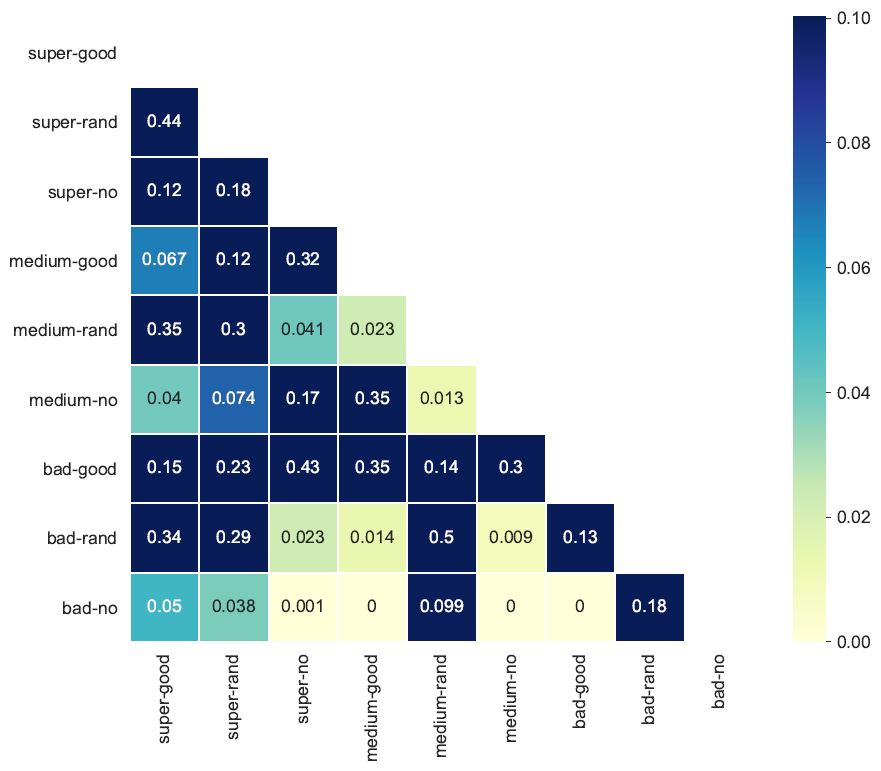
\includegraphics[width=\textwidth]{img/results_matrix_proxy_away.JPG}
			\caption{Comparison of proxy trust (away) scores ordered by classifier, value reporting difference of means ($\bar{x}_{row} - \bar{x}_{column}$ ), asterisk reporting significance (* significant at $\alpha=0.05$, ** significant at $\alpha=0.01$)}
			\label{fig:results_proxy_away}
		\end{minipage}%
		\hspace{5mm}
		\begin{minipage}[t]{0.65\textwidth}
			\centering
			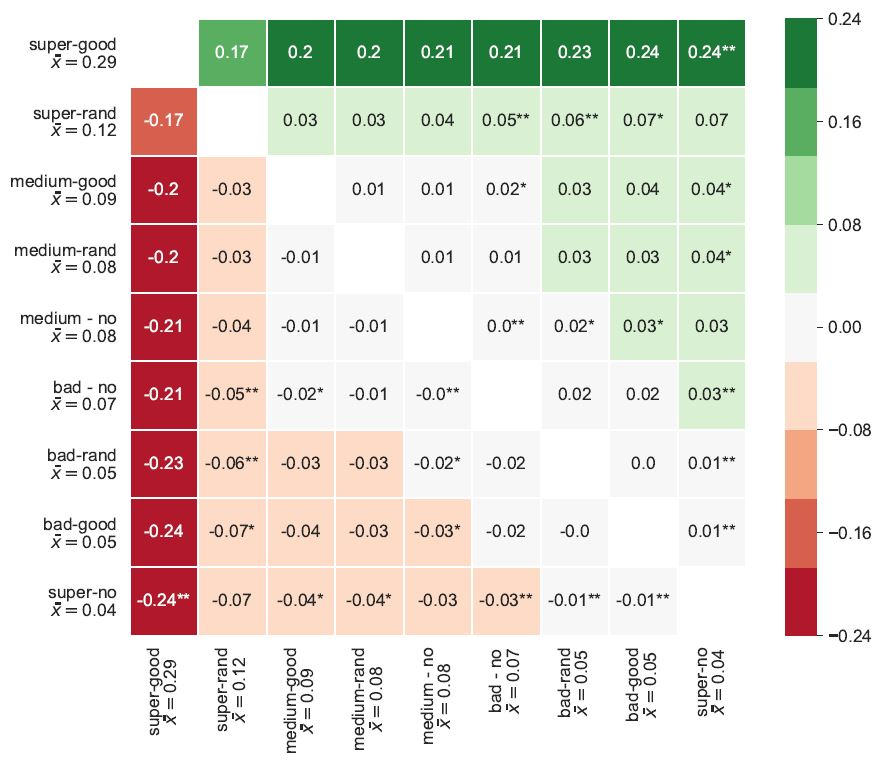
\includegraphics[width=\textwidth]{img/results_matrix_proxy_away_reordered.JPG}
			\caption{Comparison of proxy trust (away) scores ordered by explanation type, value reporting difference of means ($\bar{x}_{row} - \bar{x}_{column}$ ), asterisk reporting significance (* significant at $\alpha=0.05$, ** significant at $\alpha=0.01$)}
			\label{fig:results_proxy_away_reordered}
	\end{minipage}}
\end{figure}
\noindent Looking at the changes made towards the truth in agreement with the classifiers, no significant differences are noted between any condition with the very good and medium classifier. The same holds true for the bad classifier. The very good and medium classifiers, however, evoked significantly more changes towards the truth than the bad classifier with explanations. The standard deviations of the conditions using the bad classifier are rather high as compared to any other condition.\newline
One condition is exceptional in this analysis: Although the bad classifier without explanation has the highest mean score (i.e. changes towards the truth when the classifier made a correct prediction), the score is not significantly different from the bad classifier with a good and random explanation. The variance of all three systems (bad-no, bad-random, bad-good) are very high as compared to the variances of the other systems. The score deviates, however, from the results of the very good and medium classifier, which have lower mean scores but lower variances. The difference in variance is important to note when comparing the relatively high mean score of the bad classifier without explanation to the conditions with the very good and medium classifiers.

\begin{table}[H]
	\makebox[\textwidth][c]{
		\begin{tabular}{lrrrrrrrr}
			\textbf{Condition} & 
			\head{1.5cm}{\textbf{Total cases}} & 
			\head{1.5cm}{\textbf{Cases with opportunities}} & 
			\head{1.5cm}{\textbf{Avg opportunities}} & 
			\head{1.5cm}{\textbf{Cases with changes}} & 
			\head{1.5cm}{\textbf{Avg changes}} & 
			\head{1.5cm}{\textbf{Cases with changes towards}} & 
			\head{1.5cm}{\textbf{Avg changes towards}} & 
			\head{1.5cm}{\textbf{Norma-lised mean}} \\ \midrule
			super-good &	 30 &	 30 &	 14.53 &	 20 &	 1.40 &	 18 &	 1.07 &	 \textbf{0.07} \\
			super-rand &	 32 &	 32 &	 14.47 &	 18 &	 1.09 &	 14 &	 0.69 &	 \textbf{0.05} \\
			super-no &	 	34 &	 34 &	 14.32 &	 18 &	 1.18 &	 15 &	 0.91 &	 \textbf{0.06} \\
			medium-good &	 33 &	 33 &	 11.52 &	 17 &	 1.12 &	 12 &	 0.67 &	 \textbf{0.06} \\
			medium-rand &	 30 &	 30 &	 11.43 &	 20 &	 1.37 &	 12 &	 0.57 &	 \textbf{0.05} \\
			medium-no &	 30 &	 30 &	 11.60 &	 20 &	 1.00 &	 16 &	 0.67 &	 \textbf{0.06} \\
			bad-good &	 	38 &	 21 &	 0.55 &	 20 &	 0.95 &	 1 &	 0.05 &	 \textbf{0.05} \\
			bad-rand &	 	30 &	 22 &	 0.73 &	 19 &	 1.13 &	 1 &	 0.05 &	 \textbf{0.05} \\
			bad-no &	 	30 &	 22 &	 0.73 &	 19 &	 1.23 &	 2 &	 0.09 &	 \textbf{0.09} \\ \bottomrule
	\end{tabular}}
	\caption{Statistics for trust measure via proxy (changes towards truth and system decision)}
	\label{fig:results_table_proxy_towards}
\end{table}

\begin{figure}[H]
	\makebox[\textwidth][c]{
		\begin{minipage}[t]{0.65\textwidth}
			\centering
			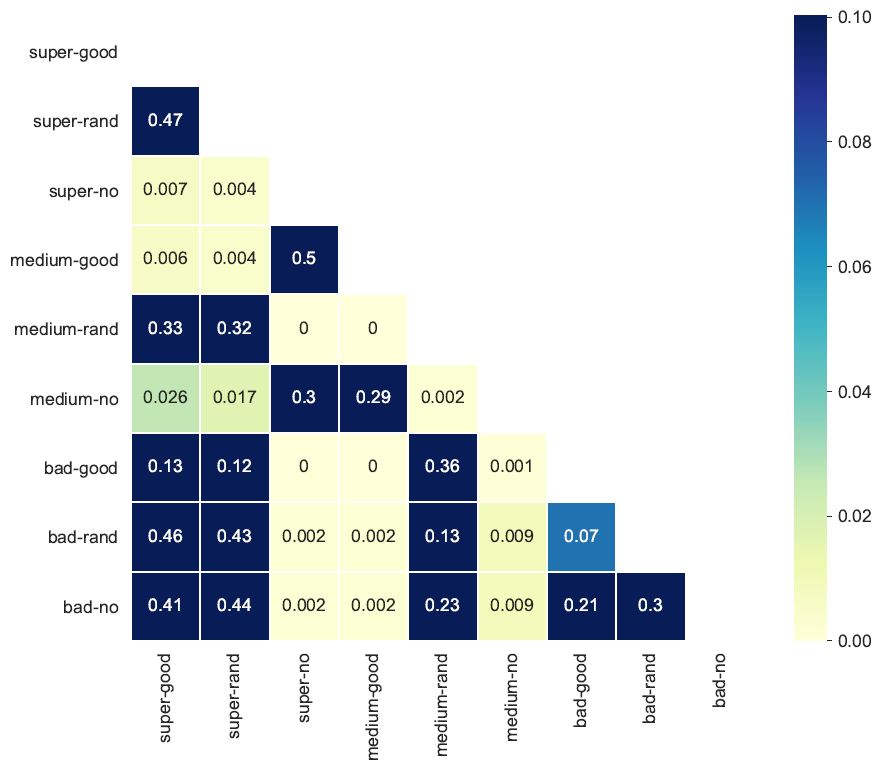
\includegraphics[width=\textwidth]{img/results_matrix_proxy_towards.JPG}
			\caption{Comparison of proxy trust (towards) scores ordered by classifier, value reporting difference of means ($\bar{x}_{row} - \bar{x}_{column}$ ), asterisk reporting significance (* significant at $\alpha=0.05$, ** significant at $\alpha=0.01$)}
			\label{fig:results_proxy_towards}
		\end{minipage}%
		\hspace{5mm}
		\begin{minipage}[t]{0.65\textwidth}
			\centering
			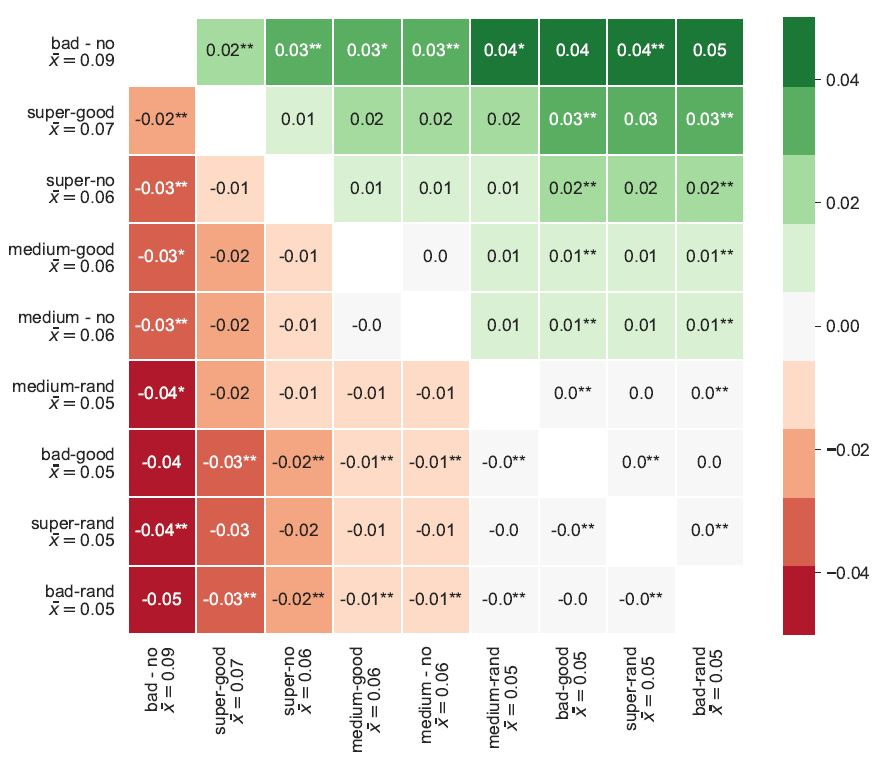
\includegraphics[width=\textwidth]{img/results_matrix_proxy_towards_reordered.JPG}
			\caption{Comparison of proxy trust (towards) scores ordered by explanation type, value reporting difference of means ($\bar{x}_{row} - \bar{x}_{column}$ ), asterisk reporting significance (* significant at $\alpha=0.05$, ** significant at $\alpha=0.01$)}
			\label{fig:results_proxy_towards_reordered}
	\end{minipage}}
\end{figure}


%\section{Discussion}
%-------------------------------------------------------------------------
% RQ 1: effect of accuracy on trust
\paragraph{Accuracy} 
Our results suggest that \textit{both perceived understanding and trust are positively related to the classifier's accuracy in general} (\textbf{RQ 1}). The higher the accuracy, the higher the trust in the system. The strongest evidence is found in the reactions to the classifiers without explanations (\textit{super-no}, \textit{medium-no}, \textit{bad-no}). The self-reported trust was the highest for \textit{super-no} and the lowest for \textit{bad-no}, with all scores differing significantly from each other. The same can be observed even when adding nonsensical explanations: The \textit{super-rand} still has significantly higher trust and perceived understanding scores than \textit{medium-rand} and \textit{bad-rand}, with the \textit{bad-rand} again having the lowest scores. The good explanation, however, influences the trust and perceived understanding differently. Here, \textit{bad-good} still receives significantly worse trust and understanding scores than both \textit{medium-good} and \textit{super-good}, yet there is no difference anymore in the scores of \textit{medium-good} and \textit{super-good}. An explanation for the similarity of both the trust score and the perceived understanding score for \textit{super-good} and \textit{medium-good} could be the persuasiveness of a good explanation. The difference in trust and perceived understanding that we see between \textit{super-no} and \textit{medium-no} could be compensated by convincing the user of the classifier's trustworthiness through a good explanation.\newline
It seems intuitive to have higher trust in a system that leads to fewer deception, which has also been described in \cite{glass2008toward} with the ``expectation mismatch" (see section \ref{subsubsec:trust_factors}). A classifier with high accuracy effectively leads to fewer disappointed expectations, which in turn does not decrease the trust. Furthermore, the set size of 15 Tweets seems to be enough for users to develop an intuition about the classifier's accuracy.\newline
%-----------------------------------------------------------------------
% RQ 2.1: presence of explanation
\paragraph{Presence of Explanations} 
In the copy machine experiment by \cite{langer1978mindlessness}, only the pure presence of an explanation was enough to make people comply with a request resulting in a short waiting time. On the basis of that experiment, we designed three explanations similar to the setup in \cite{langer1978mindlessness}: No explanation, placebic explanation, and a meaningful explanation for the classifier's behaviour. Similar to the results of the copy machine experiment, we expected to see no difference between trust scores of the meaningful and placebic explanation, but a difference between the two explanations and the no explanation settings. The results, however, lead to a different conclusion: In our experiment, \textit{the presence of an explanation did not have a positive effect on trust in any of the conditions} (\textbf{RQ 2.1}). Adding an explanation to the system influenced the trust in the very good and the medium classifier; it decreased the trust in the very good classifier and did not matter for the bad classifier. For the medium classifier, the type of explanation was crucial for its influence - a good explanation raised trust to the level of no explanation, while a nonsensical decreased trust levels.\newline
For the \textit{very good classifier}, other than expected, \textit{super-no} shows better results than \textit{super-good} and \textit{super-rand}. The classifier performed at an accuracy of 0.95, which resulted in 44\% of the cases in a perfect classification rate within the small subset of 15 Tweets. A possible explanation for the good trust score of \textit{super-no} could be the conservation of a perfect image throughout the 15 Tweets. The classifier makes (almost) no mistakes and does not offer any information that could lead to doubts about the classifier's abilities. Both \textit{super-good} and \textit{super-rand} would then have a disadvantage over the no explanation condition: The good explanations are not necessarily meaningful to a human, as they are based on statistical information rather than semantics or intentions. The placebic explanation is generated at random, which likewise holds potential for doubts and incomprehension. A similar guess was ventured in \cite{cramer2008effects}, who suspected that more knowledge about system boundaries and unfulfilled preferences leads to a decrease in trust (see section \ref{subsubsec:trust_factors}). The opposite can be observed in the proxy measure for trust, i.e. the changes in labelling that a user made towards the classifier's decision but away from the truth. Here, \textit{super-no} led to significantly fewer changes away from the truth as compared to \textit{super-good} and \textit{super-rand}, which is in turn consistent with the results in the copy machine experiment. It is important to note that the copy machine experiment only worked while people are in a ``mindless" state, i.e. an inattentive state of mind. It is possible that users did not in particular pay attention to their trust towards the system during the classification task, but actively reflected on their relationship with the system during the self-report of trust. Being in a mindless state during the proxy measurement while being mindful during the trust questionnaire would explain the conflicting results of both measures.\newline
The result for the \textit{medium classifier} differs from that of the very good classifier. The trust score of \textit{medium-no} does not differ significantly from \textit{medium-good}, but is higher than the score of \textit{medium-rand}. While the very good classifier had lower trust scores for \textit{super-good} than for \textit{super-no}, the medium classifier shows an equal trust score for good and no explanations. The medium classifier has a lower accuracy and makes three to four mistakes on each subset. It is imaginable that users are more conscious about the classifier's behaviour than they were with the (almost) perfect system due to the higher error rate. Seeing a meaningful explanation about why the classifier came to a faulty decision could raise the trust, while not seeing the reasons for a classification mistake could decrease trust - eventually ending up at the same level.\newline
The \textit{bad classifier} did not show evidence of diverting trust scores for any of the three explanation types. The same homogeneity is found in the results of the proxy measurement of trust, for both the changes away from the truth and towards the truth. The trust scores were significantly lower than any other condition, with one exemption: \textit{bad-no} had comparable trust ratings as \textit{medium-rand}. Since there is a significant distance between the scores of \textit{medium-rand} and both \textit{medium-good} and \textit{medium-no}, we conclude that it is due to a property of the medium-random system rather than a phenomenon of the bad classifier.\newline
We note that no condition with explanation leads to a significantly higher trust level than no explanation. Our findings therefore do not support the claims made in literature about a positive effect of explanations on user trust (see section \ref{subsubsec:Explanation Goals}). More drastically, if both explanation types fail to receive higher scores than no explanation, users seem to have ``blind faith" that can be harmed (but not increased) by being informed about the system. Yet, offering an explanation does not inevitably harm the user's trust. For the medium and bad classifier, the good explanation led to an equal amount of trust as no explanation. The users of the systems with good explanations, however, have knowledge about the system and potentially a more truthful mental model. If that is the case (which should be confirmed in future research), those users are more able to judge about the system in terms of fairness, flaws, or completeness.\newline
%--------------------------------------------------------------------------------
% RQ 2.2: level of truthfulness
\paragraph{Level of Truthfulness} 
Our findings furthermore show that \textit{the level of truthfulness of an explanation does not make a difference for a very good nor for a very bad classifier, set does play a role for the medium classifier} \textbf{RQ 2.2}. Only for a moderate classifier with an accuracy of 0.76 (a quite realistic score for real-life applications), the explanation fidelity is important: more truthfulness leads to more trust here.\newline
For the \textit{very good classifier}, \textit{super-good} and \textit{super-rand} led to the same trust score, while \textit{super-no} had a significantly higher trust score. As explained before, both explanation types (\textit{super-good} and \textit{super-rand}) give the opportunity to notice inconsistencies, weak explanations or contradicting evidence. In this case, the level of truthfulness does not seem to make a difference, as any explanation decreases the trust. In our experiment, we chose the ``minimum explanation" approach, only showing the relation between input features and classification result. It is possible that the resolution is not high enough to see differences in trust for \textit{super-good} and \textit{super-rand}. A more detailed explanation, explaining for example the model structure, or similar and dissimilar cases, could enhance subtle differences between the two conditions, if any.\newline
\textit{medium-good} and \textit{medium-rand}, however, have significantly different trust scores: users trust \textit{medium-good} more than \textit{medium-rand}. The medium classifier delivers faulty classifications in three to four cases out of 15, which presumably raises doubts about the system. The negative effect of placebic explanations could therefore be worsened. The ``expectation mismatch" is then twofold, with the wrong classification on the one side and the useless explanation on the other side. With the good explanations, the users receive some information about the underlying reasons for a misclassification. Even if not all information of the explanation is meaningful to a human, it delivers hints to the system's function and malfunction, possibly raising overall trust.\newline
The evidence suggests that users are not fooled by a \textit{bad classifier} and do not trust it, no matter the explanation given. There is no significant difference between \textit{bad-good} and \textit{bad-rand}. Although a plausible assumption could have been that users trust a bad classifier because it is predictable, yet do not use it as a basis for their decisions because it is not accurate. A possible topic of future work could be a distinct measure of predictability as a characteristic of trust, to examine this assumption in more detail.\newline
%--------------------------------------------------------------------------------
% RQ 3: effect of explanation types on perceived understanding
\paragraph{Perceived Understanding} 
One of the factors contributing to trust is \textit{perceived understanding}. Our findings show a negative influence of meaningless information on perceived understanding (\textbf{RQ 3}). For both the medium classifier and the very good classifier, perceived understanding was the worst when delivering placebic explanations. Although actual understanding is arguably different when comparing a case without any explanation and one with good, meaningful information, the perception of knowledge about both cases is equal here. A mechanism similar to ``expectation mismatch" could be in place for perception of knowledge. While building the mental model of the classifiers, no conflicting information have to be consolidated for the good explanation and the no explanation cases. Being confronted with random and therefore meaningless explanations forces the user to unite conflicting information in the mental model. The more conflicts appear, the lower the confidence in the mental model.\newline
For the bad classifier, perceived understanding ratings are significantly lower as for other classifiers (except for medium-random, which has a low rating as well). However, the system delivering good explanations for the faulty behaviour receives a significantly higher score than no explanation and placebic explanation cases. The positive effect of high accuracy does not hold here because the classifier performs badly on the task. Yet, as the explanations give more information about the inner workings of the classifier, it seems intuitive to evoke more confidence of understanding in this case.\newline
%--------------------------------------------------------------------------------
% Further discussions
\paragraph{Trust proxy}
The proxy measurement of trust via changes in classification between the first and second block of Tweets showed ambiguous results with high variance. For research dealing with trust in computer systems, it could be useful to measure trust not only via a questionnaire that requires reflection abilities and active processing of the relationship between user and system. In our results, we see that the proxy measure reporting the observed (hence potentially unconscious) trust does not always agree with the self-reported trust. While users of \textit{super-no} report the highest trust score, they are not as easy ``lured" to make a wrong classification as the users of \textit{super-good}. If this is due to an actual gap between actions and reflections of users, the proxy measure could be more interesting for xAI practitioners as it shows how users actually interact with a system. Using a trust measure that can be determined without the participant knowing could also serve as an additional view on user trust.\medskip \newline

%--------------------------------------------------------------------------------
% Further discussions
{\color{blue} die nächsten zwei Abschnitte noch nicht bitte}
\paragraph{Limitations \& future work}
An aspect of human-machine trust that could not be covered in this study is the evolution of trust over time. We used willingness to accept a computer-generated classification result as a proxy measure for trust and observed the changes in manual classification away from the truth in favour of the classifier's decision. For \textit{super-good}, we observed a higher value of that proxy than in any other classifier-explanation condition. The validity of those results are, however, influenced by the low number of data points: only 14 participants in \textit{super-good} had the opportunity to show such a behaviour. Other participants in the same condition had a subset with perfect classification, hence no opportunity for the classifier to misclassify and subsequently convince the user that the classification is correct nevertheless. Of those 14 participants, 4 showed the behaviour in question. This number is too small to analyse in what stage of the relationship the started to trust the classifier. For further research, it would therefore be interesting to investigate how trust develops over time: Whether users start with a high trust level and decrease the trust with every mismatch, or have a basic trust level that is increased with expectation matches and decreased with every mismatch remains to be examined in future research.\newline
Our results also do not deliver information about the proportionality of accuracy and trust level. We consider two ``extreme" cases (a very good and a very bad classifier), as well as one medium classifier with a supposedly more realistic accuracy level (0.76). In future research, more classifiers in the range between the two extremes should be investigated. We saw that for the medium classifier, the explanation type matters, but it did not for the bad classifier. From our study, we cannot determine at what accuracy level this is the case. A similar phenomenon is happening towards the upper extreme: a good explanation decreases trust for high-accuracy systems, but not for medium-accuracy systems. Determining the accuracy level at which a good explanation starts to harm user trust could be useful for practitioners.\newline
For generating explanations, we used the minimum explanation approach. The approach is limited in that it does not deliver information about the inner structure of a classifier, but only about the relation between input and output. As discussed before, examining the influence of the explanation's ``explanatory power" could give valuable information for xAI practitioners. \cite{ribeiro2018anchors} compared an explanation with little explanatory power (one if-then rule) to an explanation with more explanatory power (two if-then rules) and did not find evidence that more explanatory power leads to better understanding of the systems. Although they increased the explanation content, they only varied the amount of if-then rules instead of giving information of different kind (the classification probability, similar or dissimilar cases, the model structure, etc.).\newline

%--------------------------------------------------------------------------------
% Further discussions
\paragraph{Societal impact}
a warning sign that we need to avoid inappropriate trust in computer systems, but:
accuracy weighs strongest --> people not easy to trick
high-level study, should be tested again with actual discrimination (not easy to get the data, though)


\section{Conclusion}
This paper presents empirical evidence for the influence of accuracy and explainability on user trust. First, we generated truthful minimal explanations and nonsensical explanations for three systems with different performance levels. We then validated the explanations' fidelity by reducing sample points to input features used for the explanations, and re-classifying those sample points a second time with the same classifiers. We built a use scenario and tested the explanations in a user study. The users' trust was measured with a self-reporting questionnaire and a proxy measure based on observations of how the participants' classifications were influenced by seeing the explanations.\newline
Our findings show that users have the most trust in systems without explanations, i.e. minimum explanations can potentially harm, but not improve user trust. We argue that the act of reconciling conflicting information of the mental model and the given explanations counts as a deceptive experience and therefore affects the user's trust negatively. If an explanation is added to a system (e.g. for increasing user's understanding of the system), its truthfulness is crucial for user trust. We saw that for systems with a medium accuracy (0.76), a truthful explanation does not harm user trust, while a nonsensical explanation decreases trust. Overall, the systems' accuracy levels were most decisive for user trust: the higher the accuracy, the higher the user's trust.\newline
Further research with more rich explanations and a detailed investigation of trust factors is needed to examine potential positive effects of explanations on user trust. The development of trust over time should also be researched in the future, to give valuable directions to xAI practitioners implementing explanations in productive systems.


\bibliographystyle{plain}
\bibliography{mybib}

\section*{Appendix A}

\end{document}
